\subsection*{Teil D: Winkelsummen (20 Minuten)}

\begin{merkbox}[Winkelsummen]
    \textbf{Dreieck:} $\alpha + \beta + \gamma = 180°$\\
    \textbf{Viereck:} Summe aller Innenwinkel = 360°\\
    \textbf{n-Eck:} Summe aller Innenwinkel = $(n-2) \cdot 180°$
\end{merkbox}

\begin{enumerate}[label=\arabic*., resume]

    \item \textbf{Berechne die fehlenden Winkel im Dreieck:}

    \vspace{0.5cm}

    \begin{center}
        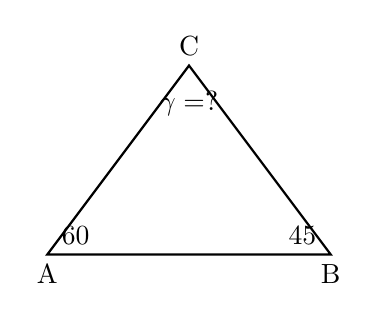
\begin{tikzpicture}[scale=1.2]
            \draw[thick] (0,0) -- (3,0) -- (1.5,2) -- cycle;
            \node at (0.3,0.2) {$60°$};
            \node at (2.7,0.2) {$45°$};
            \node at (1.5,1.6) {$\gamma = ?$};
            \node[below] at (0,0) {A};
            \node[below] at (3,0) {B};
            \node[above] at (1.5,2) {C};
        \end{tikzpicture}
    \end{center}

    $\gamma = 180° - 60° - 45° = $ \underline{\hspace{3cm}}

    \vspace{1cm}

    \item \textbf{Berechne alle Winkel im gleichschenkligen Dreieck:}

    \vspace{0.5cm}

    Gegeben: Gleichschenkliges Dreieck mit Basiswinkeln von je 70°.

    \begin{center}
        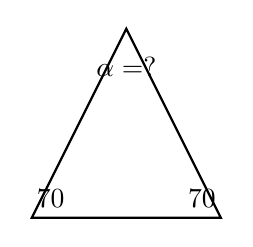
\begin{tikzpicture}[scale=1.2]
            \draw[thick] (0,0) -- (2,0) -- (1,2) -- cycle;
            \node at (0.2,0.2) {$70°$};
            \node at (1.8,0.2) {$70°$};
            \node at (1,1.6) {$\alpha = ?$};
        \end{tikzpicture}
    \end{center}

    $\alpha = $ \underline{\hspace{3cm}}

    \vspace{1cm}

    \item \textbf{Berechne die Winkelsumme im Fünfeck:}

    \vspace{0.5cm}

    Formel: Winkelsumme = $(n-2) \cdot 180°$

    Für $n = 5$: Winkelsumme = $(\phantom{0}-2) \cdot 180° = \phantom{0} \cdot 180° = $ \underline{\hspace{3cm}}

    \vspace{1cm}

    \item \textbf{Komplexere Aufgabe:}

    In einem Viereck ABCD sind drei Winkel bekannt: $\angle A = 85°$, $\angle B = 95°$, $\angle C = 110°$.

    Berechne $\angle D$:

    $\angle D = 360° - 85° - 95° - 110° = $ \underline{\hspace{3cm}}

    \vspace{1cm}

    \item \textbf{Bonusaufgabe:}

    Beweise, dass die Winkelsumme im Dreieck 180° beträgt:

    \begin{center}
        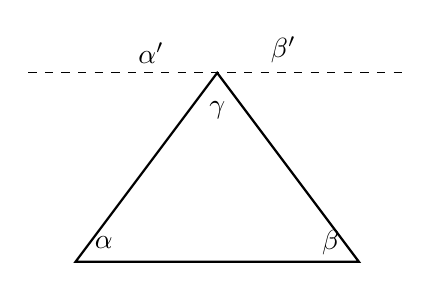
\begin{tikzpicture}[scale=1.2]
            \draw[thick] (0,0) -- (3,0) -- (1.5,2) -- cycle;
            \draw[dashed] (-0.5,2) -- (3.5,2);
            \node at (0.3,0.2) {$\alpha$};
            \node at (2.7,0.2) {$\beta$};
            \node at (1.5,1.6) {$\gamma$};
            \node[above] at (0.8,2) {$\alpha'$};
            \node[above] at (2.2,2) {$\beta'$};
        \end{tikzpicture}
    \end{center}

    Die gestrichelte Linie ist parallel zur Grundseite.

    Begründung: \underline{\hspace{8cm}}

    \underline{\hspace{10cm}}

\end{enumerate}